
\chapter{Metodologia\label{chap:Metodos}}

% Resumo opcional. Comentar se não usar.
%\resumodocapitulo{resumo}


\section{Materiais}
\subsection{Hardware}
\subsubsection{Leitora RFID Impinj Speedway R420}

A Speedway R420 da fabricante Impinj é uma pequena leitora estacionária de \textit{tags} de RFID passivo. Ela é capaz de operar na faixa de frequência de 860-960 MHz, sendo que o modelo específico licenciado para o Brasil permite operações entre 902,5 e 907 MHz. Pode emitir sinais de até 32,25 dBm de potência na transmissão e é capaz de receber um sinal com a sensibilidade mínima de -80 dBm e perda de retorno de 10 dB \cite{SpeedwayRDatasheet} \cite{SpeedwayRUserManual} \cite{TG2013OliveiraERocha}. A figura \ref{fig:SpeedwayR420_first} mostra uma foto da leitora.

    \begin{figure}[H]
        \centering
        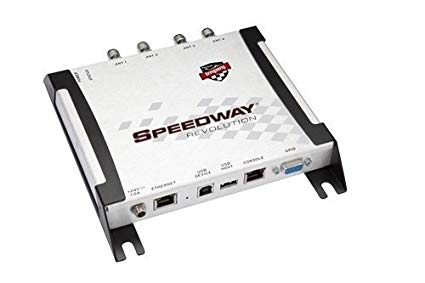
\includegraphics[width=0.55\linewidth]{figs/Metodologia/leitoraSpeedwayR420.jpg}
        \caption{Leitora Impinj Speedway R420 \cite{SpeedwayRUserManual}}
        \label{fig:SpeedwayR420_first}
    \end{figure}

 A leitora é capaz de registrar até 1100 etiquetas por segundo. Ela possui portas suficientes para o acoplamento de até 4 antenas, expansível até 32 antenas utilizando \textit{Hubs} específicos para esta aplicação. Dois protocolos são utilizados para a interface por ar: \textit{GS1/EPCglobal UHF Gen2 (ISO 18000-6C)} e \textit{RAIN RFID} \cite{SpeedwayRDatasheet}\cite{SpeedwayRUserManual}. As portas de conexão das antenas podem ser vistas na figura \ref{fig:SpeedwayR420front}.
 
     \begin{figure}[H]
        \centering
        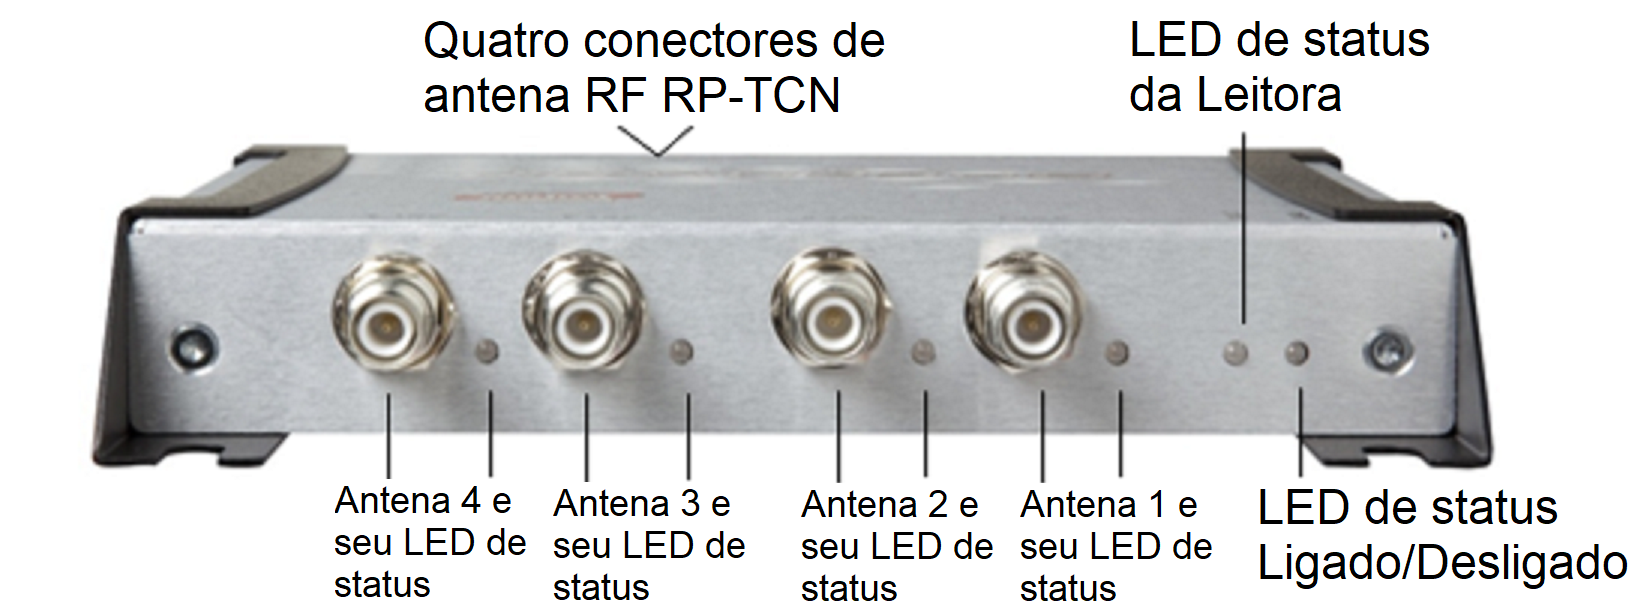
\includegraphics[width=0.6\linewidth]{figs/Metodologia/SpeedwayR420-front-view.png}
        \caption{Leitora Impinj Speedway R420 - vista frontal \cite{SpeedwayRUserManual}.}
        \label{fig:SpeedwayR420front}
    \end{figure}
 
 Existem diversas portas na parte traseira da leitora Speedway R420. Uma delas é uma porta \textit{10/100 BaseT Ethernet} para comunicação em TCP/IP. A comunicação por TCP/IP é ideal para o uso comum, utilizando os softwares comercializados pela Impinj ou por programas feitos utilizando o pacote \textit{Impinj OctaneSDK}. Além dessa porta, a comunicação pode ser feita por USB ou por comunicação serial RS-232 em um conector RJ45 para acesso ao console embarcado na leitora. As portas seriais são ideais para utilização dos pacotes \textit{Impinj LTK} de programação em baixo nível, utilizando o padrão \textit{Low Level Reader Protocol} (LLRP). Baixo nível, neste caso, implica capacidade de alterar o protocolo de operação, o modo de marcação de tempo e dos parâmetros de comando por ar\cite{GS1-LLRP}\cite{SpeedwayRUserManual}. A visão traseira da leitora é apresentada na figura \ref{fig:SpeedwayR420back}.
 
\begin{figure}[H]
    \centering
    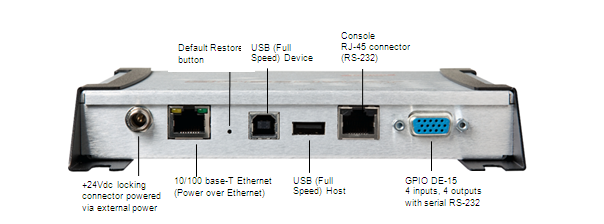
\includegraphics[width=0.6\linewidth]{figs/Metodologia/SpeedwayR420-back-view.png}
    \caption{Leitora Impinj Speedway R420 - vista traseira - Foto obtida no manual de instalação e operação da leitora \cite{SpeedwayRUserManual}.}
    \label{fig:SpeedwayR420back}
\end{figure}
 
 Existe ainda uma porta \textit{GPIO DE-15} (\textit{General Purpose Input-Output DE-15} - Porta de uso de próstio geral para entrada e saída de dados)\cite{SpeedwayRUserManual}. Ela pode ser utilizada para a configuração de comandos e gatilhos de leitura.
 
 A alimentação elétrica da leitora pode ser feita utilizando o padrão \textit{PoE} (\textit{Power over Ethernet}) \cite{SpeedwayRUserManual}, ou seja, sem a necessidade de fonte externa, apenas através do cabo Ethernet, ou então pode ser feita com uma fonte 24 volts de corrente contínua \cite{IEEE-SA-POE}. A fonte pode prover uma confiabilidade maior para operação com potências maiores, próximas ao limite de 32,25 dBm, enquanto a alimentação \textit{PoE} permite maior flexibilidade na instalação do produto, principalmente em relação à passagem de cabos e instalação de tomadas.
 
 \subsubsection{Antena RFID Impinj Threshold}
 
 A Threshold, também da fabricante Impinj, é uma antena RAIN RFID específica para detectar cruzamento de barreiras e fronteiras. O seu corpo alongado, com polarização linear paralela ao menor eixo, permite uma ampla cobertura, e a possibilidade de conectar múltiplas antenas para criar uma "cortina" de cobertura RFID \cite{AntenaThresholdDatasheet}.A antena pode ser vista na figura \ref{fig:AntenaThreshold_first} a seguir.
 
 \begin{figure}[H]
    \centering
    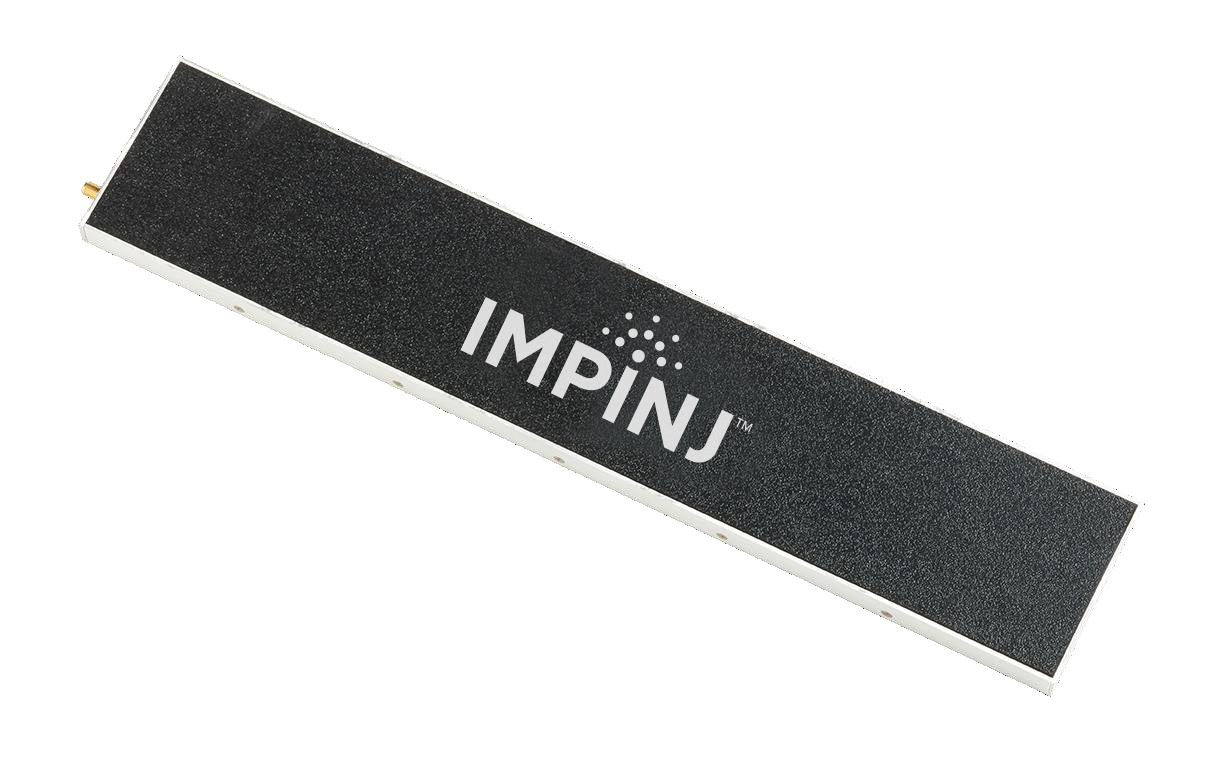
\includegraphics[width=0.5\linewidth]{figs/Metodologia/impinj_Threshold.png}
    \caption{Antena Impinj Threshold - Foto obtida no \textit{datasheet} da antena \cite{AntenaThresholdDatasheet}}
    \label{fig:AntenaThreshold_first}
\end{figure}
 
 A antena opera em duas faixas de frequência: 902-928 MHz (FCC) e 865-868 MHz (ETSI), possui um ganho de campo distante de 5.0 dBi e impedância nominal de 50 $\Omega$ \cite{AntenaThresholdDatasheet}. A antena cobre um volume elipsoidal de 3m de comprimento por 4m de largura por 3m de altura, como pode ser visto na figura \ref{fig:AntenaThresholdCobertura}.
 
  \begin{figure}[H]
    \centering
    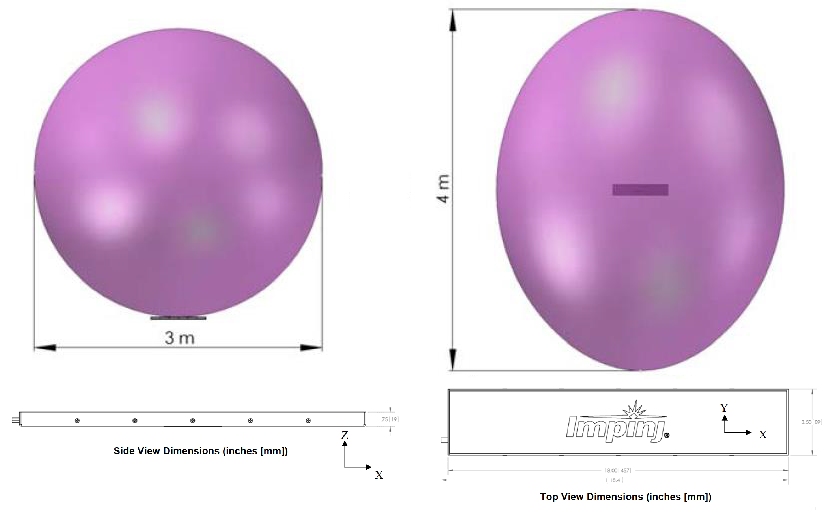
\includegraphics[width=0.6\linewidth]{figs/Metodologia/impinj_antenna_coverage.png}
    \caption{Gráfico da zona de cobertura das antenas Impinj Threshold e desenho mecânico da leitora em pontos de vista iguais aos dos desenhos de cobertura acima - Adaptado do \textit{datasheet} da antena \cite{AntenaThresholdDatasheet}}
    \label{fig:AntenaThresholdCobertura}
\end{figure}

\subsubsection{TAG utilizada no projeto}

As TAGs utilizadas são impressas em adesivos pela empresa Nycti BR. Elas utilizam chip Alien Higgs-3 RFID IC. Como características principais estão:

\begin{itemize}
    \item Banda de operação de 915-868 Mhz;
    \item Tamanho 96 X 23mm;
    \item Alcance de leitura de acordo com o fabricante de 6m (com testes empíricos feitos nas TAGs utilizadas de alcance de mais de 10m);
    \item 800-bit de memória, sendo 96 bits para armazenar o EPC - extensível até 480 bits - e 512 bits de uso de propósito geral; \cite{AlienHiggs3}
    \item ativado em baixíssimas potências de alimentação, ainda provendo excelente sinal de resposta de retroespalhamento. \cite{AlienHiggs3}
\end{itemize}

A figura \ref{fig:TAGsused} a seguir mostra as TAGs utilizadas para monitorar o trânsito das pessoas no interior dos ambientes pre-estabelecidos.

 \begin{figure}[H]
    \centering
    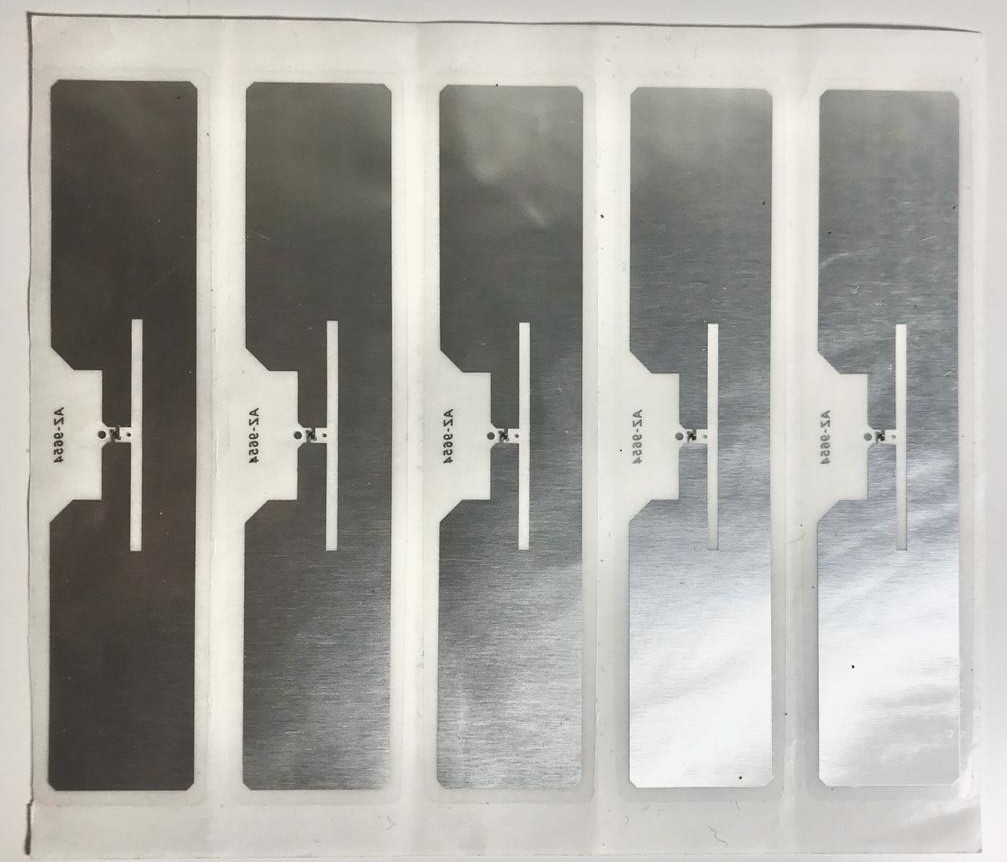
\includegraphics[width=0.8\linewidth]{figs/Metodologia/TAGsRFID.jpeg}
    \caption{TAGs utilizadas para a execução deste trabalho}
    \label{fig:TAGsused}
\end{figure}
 
 Estas TAGs mostradas na figura \ref{fig:TAGsused} foram distribuídas entre as pessoas designadas para testar o sistema criado. %TODO
 
 \subsubsection{Quantitativo}
 
 Este trabalho conta com leitoras e antenas RFID, além do espaço para trabalho e testes, gentilmente cedidos pelo Laboratório de Automação e Robótica (LARA) da UnB. No que se refere aos equipamentos, foram utilizados com os seguintes dispositivos:
 
 \begin{itemize}
     \item 3 (três) Leitoras IMPINJ Speedway R420 (cedidas pelo LARA)
     \item 6 (seis) Antenas IMPINJ Treshold (cedidas pelo LARA)
     \item 1 (um) hub DLINK 6 portas Ethernet
     \item 20 (vinte) TAGs RFID 915 MHZ
     \item cabeamento e fontes de alimentação necessários
 \end{itemize}
 
 \subsection{Software}
 
 \subsubsection{OctaneSDK}
 
 O pacote de desenvolvimento OctaneSDK para dispositivos RAIN RFID, da Impinj, foi utilizado para desenvolver a parte de software deste trabalho. O pacote possui versões para .NET e Java \cite{OctaneSDK}. O pacote para .NET foi lançado há mais tempo e possui mais versões, e, por conseguinte, mais defeitos foram corrigidos, o que torna esta implementação mais robusta do que o pacote em Java. Por esse motivo, foi escolhido para o desenvolvimento desse trabalho.
 
 \subsubsection{Visual Studio}
 
 O pacote OctaneSDK .NET foi desenvolvido para funcionar com o Ambiente Integral de Desenvolvimento (\textit{Integrated Development Environment} - IDE) Visual Studio, da Microsoft. A IDE foi utilizada para instalar o pacote de extensão do OctaneSDK. \cite{OctaneSDK}
 
 A linguagem de programação mais recomendada para desenvolvimento usando OctaneSDK com o Visual Studio é C\#. O desenvolvimento em outras linguagens baseadas em .NET \textit{framework} é possível, mas sem suporte da Impinj.

 
 \section{Abordagem utilizada}
 
 Três pontos foram essenciais para a execução deste trabalho: a implementação física das leitoras, antenas e demais equipamentos no local de teste; o \textit{software} de detecção de pessoas e cruzamento de fronteiras para a contagem de pessoas em um determinado ambiente;  e a elaboração de casos de teste para  validação da abordagem. Estes pontos serão descritos nas seções a seguir.
 
  
 \subsection{Implementação física}
 
 As leitoras e as antenas utilizadas neste trabalho possuem um grande campo de cobertura relativo a outros modelos de equipamentos RFID passivo. Entretanto, a cobertura de sinal anunciada pelo fabricante é válida para ambientes abertos e sem a presença de objetos que possam interferir no sinal, como: mesas, cadeiras, equipamentos e pessoas.
 
 A interferência de sinais de radiofrequência por metais e líquidos  é um problema conhecido na indústria. Levando em consideração este problema, um cenário fictício de um ambiente de trabalho é considerado, baseado em escritórios e laboratórios reais. Supõe-se que todos os trabalhadores e visitantes, carreguem consigo crachás de identificação, nos quais estão embutidos transpônderes RFID já existentes, utilizados no sistema de controle de acesso do escritório ou laboratório.
 
 As pessoas que transitam neste ambiente utilizam seus crachás em cordões dependurados no pescoço. Cada crachá permanece próximo ao corpo do seu usuário, porém não preso a ele. Os crachás ficam na altura do tórax.
 
 \subsection{O local}
 

 O Laboratório de Automação e Robótica (LARA) foi o local para simulação do ambiente de teste do sistema criado, especificamente, a metade sul do laboratório, onde se encontram os ambientes de estudo geral e a sala de reuniões.
 
 Esta parte do laboratório foi subdividida em quatro ambientes: o Ambiente Externo (0), a Sala Principal (1), Sala de Reuniões (2) e o Corredor de Baias (3), como pode ser observado na planta baixa da figura \ref{fig:LARA_planta}.

  \begin{figure}[H]
    \centering
    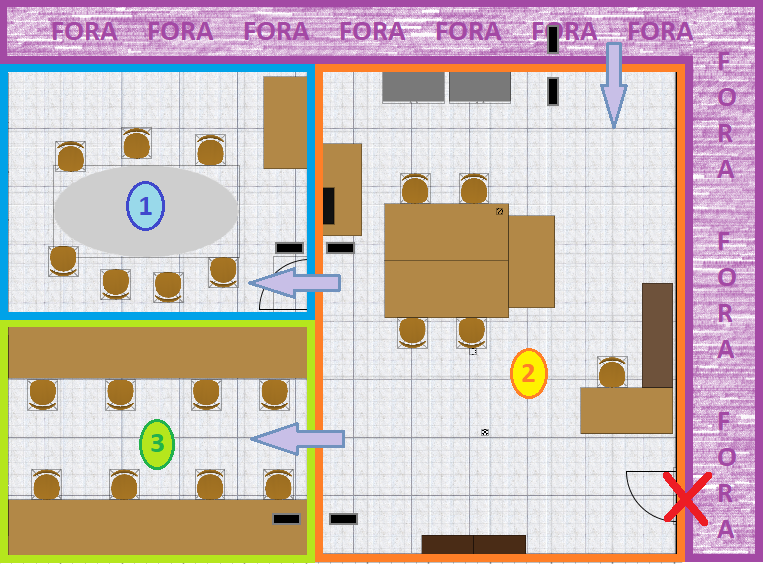
\includegraphics[width=0.9\linewidth]{figs/Metodologia/LARA_planta_ambientes.png}
    \caption{Imagem apresentando a planta baixa do LARA - local de instalação das leitoras}
    \label{fig:LARA_planta}
\end{figure}

O ambiente do laboratório pode ser melhor visualizado nas figuras \ref{fig:LARA1} e \ref{fig:LARA2} abaixo. As figuras mostram as projeções tridimensionais do laboratório, a partir de dois pontos de vista diferentes, para melhor compreensão do ambiente de estudo.

  \begin{figure}[H]
    \centering
    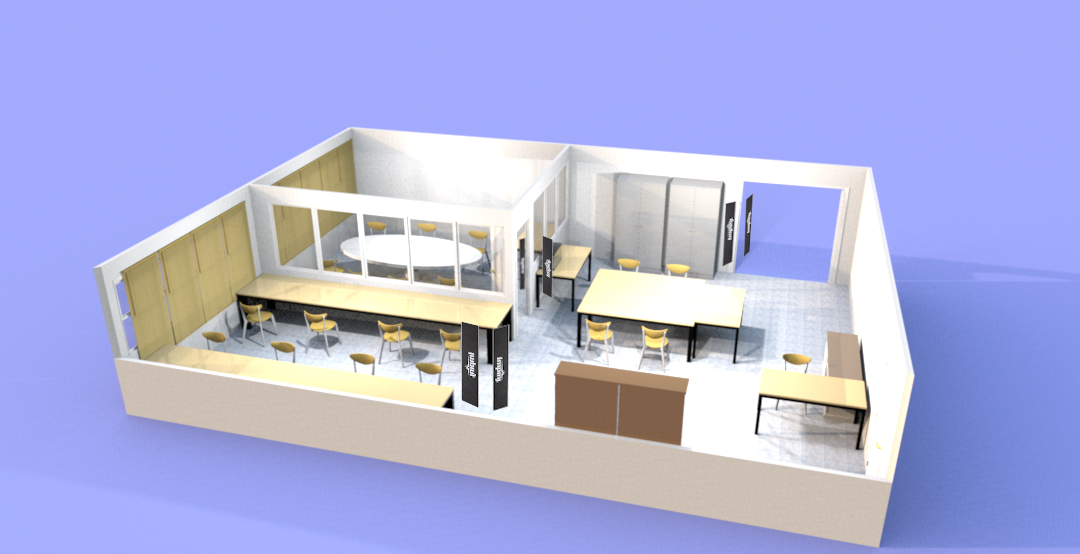
\includegraphics[width=1\linewidth]{figs/Metodologia/LARA_leitoras-1.png}
    \caption{Imagem apresentando a renderização tridimensional do LARA e o local de instalação das leitoras}
    \label{fig:LARA1}
\end{figure}

  \begin{figure}[H]
    \centering
    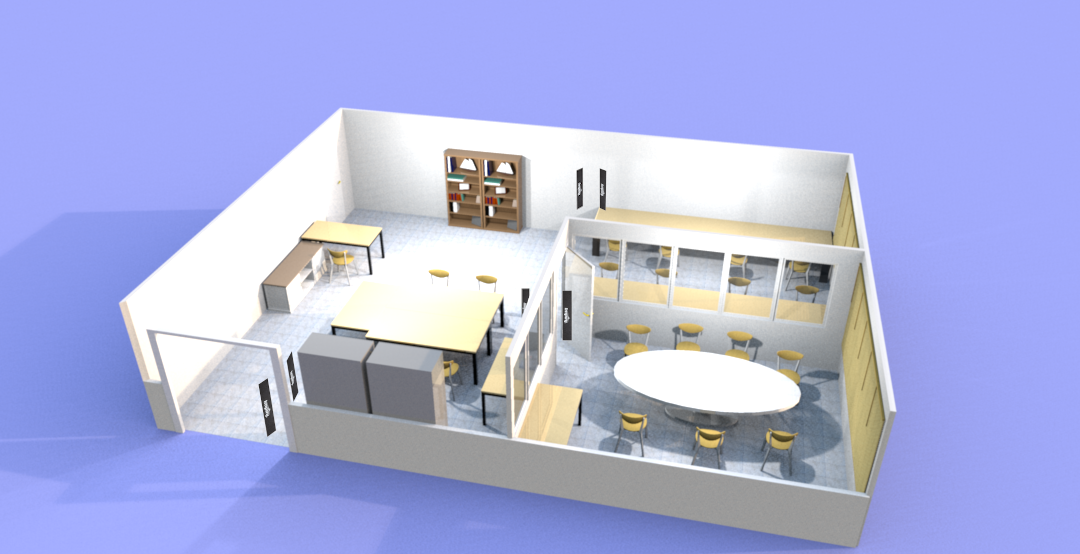
\includegraphics[width=1\linewidth]{figs/Metodologia/LARA_leitoras-2.png}
    \caption{Imagem apresentando a renderização tridimensional do LARA a partir de um segundo ponto de vista - local de instalação das leitoras}
    \label{fig:LARA2}
\end{figure}

As três leitoras foram designadas para tratar os dados das transições. A leitora 1 (L1) trata os dados da transição entre o Ambiente Externo (0) e a Sala Principal (1); a Leitora 2 (L2) é responsável por capturar os dados da transição entre a Sala Principal (1) e a Sala de Reuniões (2); a Leitora 3 registra os cartões que passam pela transição entre a Sala Principal (1) e o Corredor de Baias (3). Cada leitora é representada por um retângulo cinza na figura \ref{fig:LARA_planta} e possui duas antenas para registrar as \textit{tags} que passam na região.

As antenas foram dispostas em locais estratégicos para se obter as leituras mais precisas, nos locais de transição de interesse. Estes locais estão localizados próximos às portas ou passagens onde estão as fronteiras dos ambientes definidos. As antenas podem ser vistas como retângulos pretos de borda cinza na figura \ref{fig:LARA_planta} e pelo desenho da leitora real nas figuras \ref{fig:LARA1} e \ref{fig:LARA1}.

As leitoras da transição entre os ambientes Sala Principal (1) e Sala de Reuniões (2) e da transição entre os ambientes Sala Principal (1), Corredor de Baias (3) foram instaladas em posições opostas da sala para minimizar a ocorrência de leitura das \textit{tags} pelas duas leitoras ao mesmo tempo.

 \subsection{Elaboração do Software}
 
 A tecnologia RAIN RFID, geralmente utilizada para aplicações de \textit{IoT} (Internet das coisas - \textit{Internet of Things} em inglês), exige a implementação de um \textit{software} para conectar os dados das TAGs registrados pelas leitoras RFID às aplicações de alto nível e de computação em nuvem, como pode ser observado na figura \ref{fig:RFID-Middleware} do capítulo anterior, sessão \ref{section: RFID}.
 
 A estratégia utilizada foi baseada na estratégia
 

 
 
 \begin{figure}[H]
    \centering
    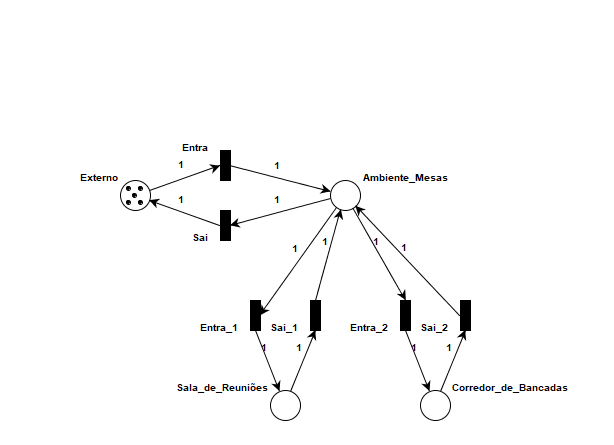
\includegraphics[width=0.8\linewidth]{figs/Metodologia/Petri_net.png}
    \caption{Rede de Petri representando todas as possibilidades circulação de pessoas pelo LARA como estados e transições}
    \label{fig:Petri1}
\end{figure}

 \begin{figure}[H]
    \centering
    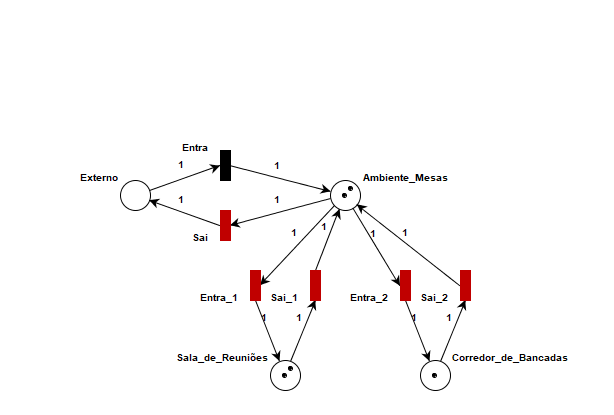
\includegraphics[width=0.8\linewidth]{figs/Metodologia/Petri_net2.png}
    \caption{Rede de Petri representando a circulação de pessoas pelo LARA em um caso hipotético}
    \label{fig:Petri2}
\end{figure}
 
 

 
 
 
 
 \subsection{Casos de teste}
 
